%!TEX root = ../dissertation.tex
\chapter{Conclusions and Future Works}
\label{conclusion}

We conclude this work making some consideration on the obtained results with the presented algorithms for sentiment analysis on Italian automotive forums. Along with these results, we propose some improvements to enhance the performance of the models in order to make the future results more reliable. Finally, will be proposed a solution in order to integrate this sentiment analysis tool in a real world case.

\section{Results of the Sentiment Analysis Models}

The goal of this work was to apply sentiment analysis to the automotive dataset, on online Italian forums comments. The chosen strategies involved machine learning approaches, and since it does not already exist suitable datasets, the first approach was to collect one. With some manually designed scripts, have been crawled some popular forums, obtaining almost 1,200,000 comments. Even if the subject of the sentiment was a particular manufacturer, comments have been taken from every discussion of any manufacturer, in order to inject some noise, which is useful to avoid biases. From a preliminary look at the topic most treated into the forums, has been selected a list of arguments, for which every comment must be labeled, selecting a sentiment polarity between "very positive", "positive", "neutral", "negative" and "very negative", plus an additional "irrelevant" for saying that in the comment the argument is not treated. In a second moment, the polarities were grouped into a three-degrees sentiment scale. All tests were made for the class "engine", since is is one of the most populated (even if not plenty of data at all), and with explicit references to the engine, that are supposed to make the classification easier.\\
In this work it has been designed a two-stages cascade classifier, in all its parts, and it was compared with a one-step classifier, for detecting the pertinence about some topics and eventually the sentiment of automotive comments.\\
Before starting with the crawled dataset, have been made some tests on a sentiment analysis Twitter's dataset, that actually show great performance compared to the state of the art. A baseline approach involving \acl{SVM} classifier reached around 70\% accuracy, which is a remarkable result, but improved with the designed revised \acl{BPEF} model, that reached around 75\% accuracy, which is close to state of the art results. In all cases, features selection improved the overall performance, which means that the used techniques were able to select most important components that carried the sentiment information. These experiments served as benchmark to test the goodness of the implementation of the model, before to design the main model for the Italian dataset. Our implementation actually simplified the original \ac{BPEF} system, by the fact that dataset parameters were not explicitly implemented (because intrinsic in the dataset creation), and the model selection algorithm that has not been implemented, due to the few trained classifiers. Even these simplifications, the model reached the mentioned good results, that suggest that the whole implementation should just make some eventual little improvements on the scores.\\
When it was shown that implemented models worked, it was designed a baseline approach for classification of the "engine" class, and then an improved cascade classifier. The first reached poor results, due to the lack of comments, but mostly because of the high imbalances to the "irrelevant" class that inducted a high bias, that made the "negative" polarity ignored at all. For this reason, the idea to split the overall classification into two stages: a first that detects if an argument is treated, and the second that classifies the sentiment. Splitting the problems into two phases, the two classifiers can be trained with less imbalance classes, and the performance showed a big improvement: the scores present a huge improvement with respect to the baseline approach, but most importantly the reliability of the solution. With these facts, the choice of splitting the problem into two smaller ones was the right one for this problem.\\
The same model was trained for the classification of other classes: "brand", "exteriors" and "support". The choice fell on these three other arguments, because the most relevant for a car manufacturer, but obviously the same approach can be extended to all other topics. The scores show better performance on the "engine" class, mostly due to the relevance detection, that worked better on this class. The reason can be associated to the quantity of the relevant comments, that is higher than the other classes (except for "brand"), and to the fact that comments related to the engine, generally have explicit references, so easier to interpret. In fact, even if the "brand" class has more data than "engine", lot of reference to the brand in the comments are actually implicit, and hard to interpret.\\
Another consideration regards the imbalances. Every class have data imbalances, and due to the lack of comments, it is not suggested to cut the dataset in order to get the balance. This issue makes the classifier biased to the majority polarity, and it is visible for instance in Figure \ref{fig:ita_cascade_support_bpef_val}, where since the data are especially "negative", the classifier tend exactly to predict this polarity.


\section{Enhancements}

As previously said, the final results show good performance, but there are some ways to improve the classifications. Supposing further enhancements, the system should make more reliable classifications, so decisions based on data should be more confident.\\
The main focus about enhancements regards the dataset, which is the main responsible for a poor representation of the real world. The main strategies to go trough will be:
\begin{itemize}
	\item Dataset extension;
	\item Comments' information gathering;
	\item Dataset labeling.
\end{itemize}

Extending the dataset with other data may improve the variance of the argument treated and maybe other common says, which should help the classifiers. Moreover, the presented dataset lacks especially on some topics, for instance "electrical mobility", which nowadays is really important. Supposing to gather a larger dataset, the main problematic regards the labeling. For resources constraints (mostly time) the dataset annotation was made reserving a time window to label as much comments as possible. Also for other constraints labeling was made by few improvised annotators. Supposing to have the needed resources, it will be possible to achieve more labeled data, and quality of the annotations. As shown, sometimes annotations depend on the point of view of the person rather than an objective choice, so different annotators may answer different choices. A solution for this issue may be sending all comments to multiple operators, and keeping only annotations that reached the majority choice. This solution uses a lot of resources, but hopely it will get more reliable annotations.\\
Again, supposing to have lot of annotated data, it will be possible to balance the data in order to reduce the biases that have been discussed earlier. Moreover, having more data, classifiers have should improve their performance, but in the extreme case that data are really plenty, it will be possible to test other more powerful classification algorithms, such as Neural Networks.\\
One case on which the discussed models lack is on comments that express comparisons. The main motivation is that dataset was not thought f	or these situations: in the annotations was asked to select the subject of the text, and the sentiments expressed with respect to this subject, but in the case of several subjects (like in the comparisons) the approach was to select just the main one, for instance the one of the discussion's title. Changing the approach, for instance storing the labeling information into a more flexible data format, like JSON (JavaScript Object Notation) or XML (eXtensible Markup Language). Having data collected in this sort of files, it will be possible to design better models also for handling comparisons.\\
Finally, a little consideration on some classification algorithms that have been used. Simplifying, the algorithms based on linear models actually search some weights to attach to the words that compose the sentences. The combination of the multiplicity and the actual weights gives the result of the classification. The problem is that relationship information between words are not kept, with the only exception of the N-grams. Also for this reason, some non-linear models such as Neural Networks may have the capability to detect useful relationships between words (or in general, features), and may output more reliable models.


\section{Real World System}

The presented work done until now represents just a prototype of a bigger system. In this section it will be proposed a brief explanation of a solution for a production sentiment analysis system. The system is composed by many parts, visually summarized in Figure \ref{fig:real-world-tool}.

\begin{figure}[H]
	\centering
	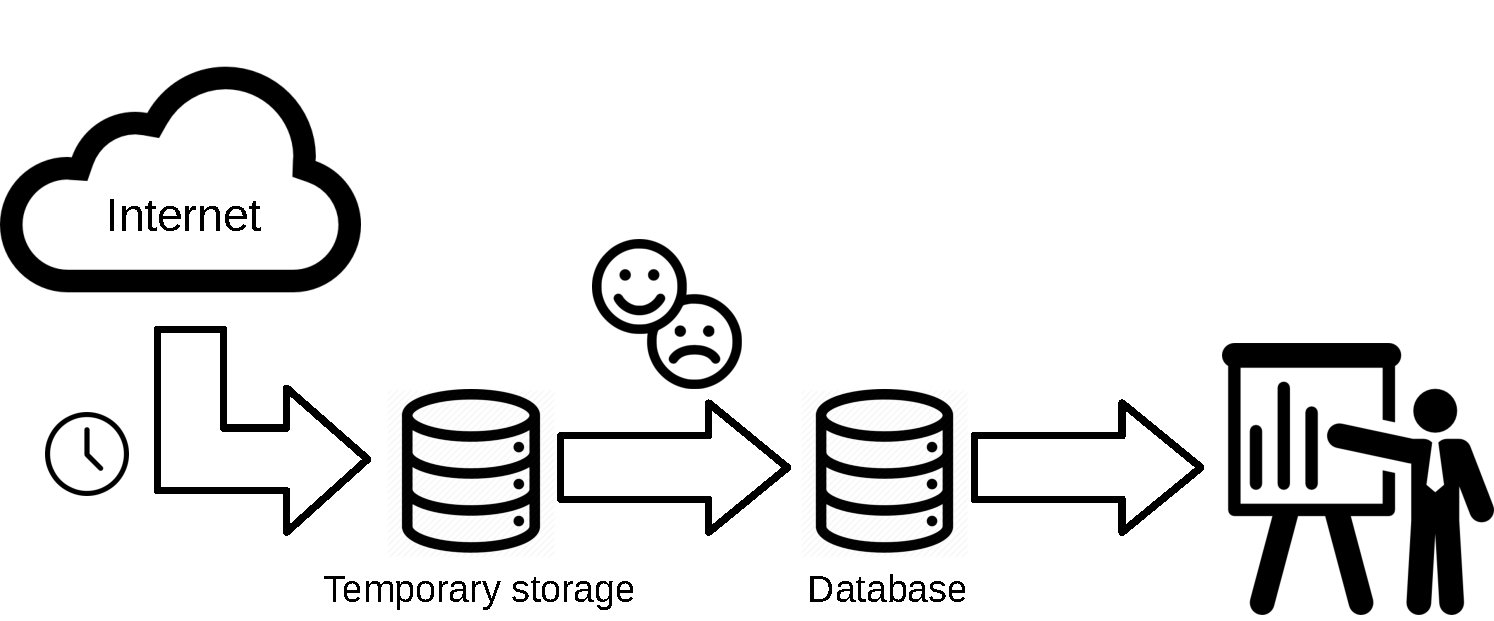
\includegraphics[width=\textwidth]{figures/real-world-tool.pdf}
	\caption{Workflow in a real world production case.}
	\label{fig:real-world-tool}
\end{figure}

A first block consists in a scheduled crawler, which is responsible to download at any period of time (for instance, once at day), all new comments found in some selected forums. Comments should be picked from every discussion of every car manufacturer, as made for the dataset creation, but with a different purpose: for dataset creation, this choice was made for injecting some noise into the data, while for the production case, it should be done for acquire comments related to the target car brand, even in discussions not related to it. All crawled comments will be then gathered in a temporary storage, that can be either a database or a file system. From there, all new comments should then annotated with the designed sentiment analysis model, with the integration of a subject detector that will be used to catch just relevant comments for what concerns the target brand's interests. Sentiment analysis model should also be integrated with the classifiers of all the initially found topics, and not just the four discussed ones, in order to make more specific analyses. This process should work again in a scheduled way, or start immediately after the end of the crawl, and it should take the comments from the temporal storage, and save the annotated data into a database, in order to make a simple integration with business intelligence tools. Finally, the data visualization tool, such as the one utilized in this work in chapter \ref{industrial-use-case}, should be used to extract useful information from the data, to make graphical dashboards, in order to make simple and easy to understand presentations.

